\newpage
\section{Test 5}
\label{Sec:test_5}

In the fifth test setting rover is dropped onto the inclined plane.
Inclination angle of the slope has been set to 10$^\circ$. After 5$^{th}$ second of motion a simple PD controller
is set on in order to stop the rover on the slope. Rover stops effectively at $t = 119.965s$. At $t = 200s$ constant torques has been applied to all the wheels.
Values of applied torques equaled $\tau = 9500Nm$. Hence, Since $t = 200s$ rover drives upwards. 

\begin{figure}[H]
  \centering
    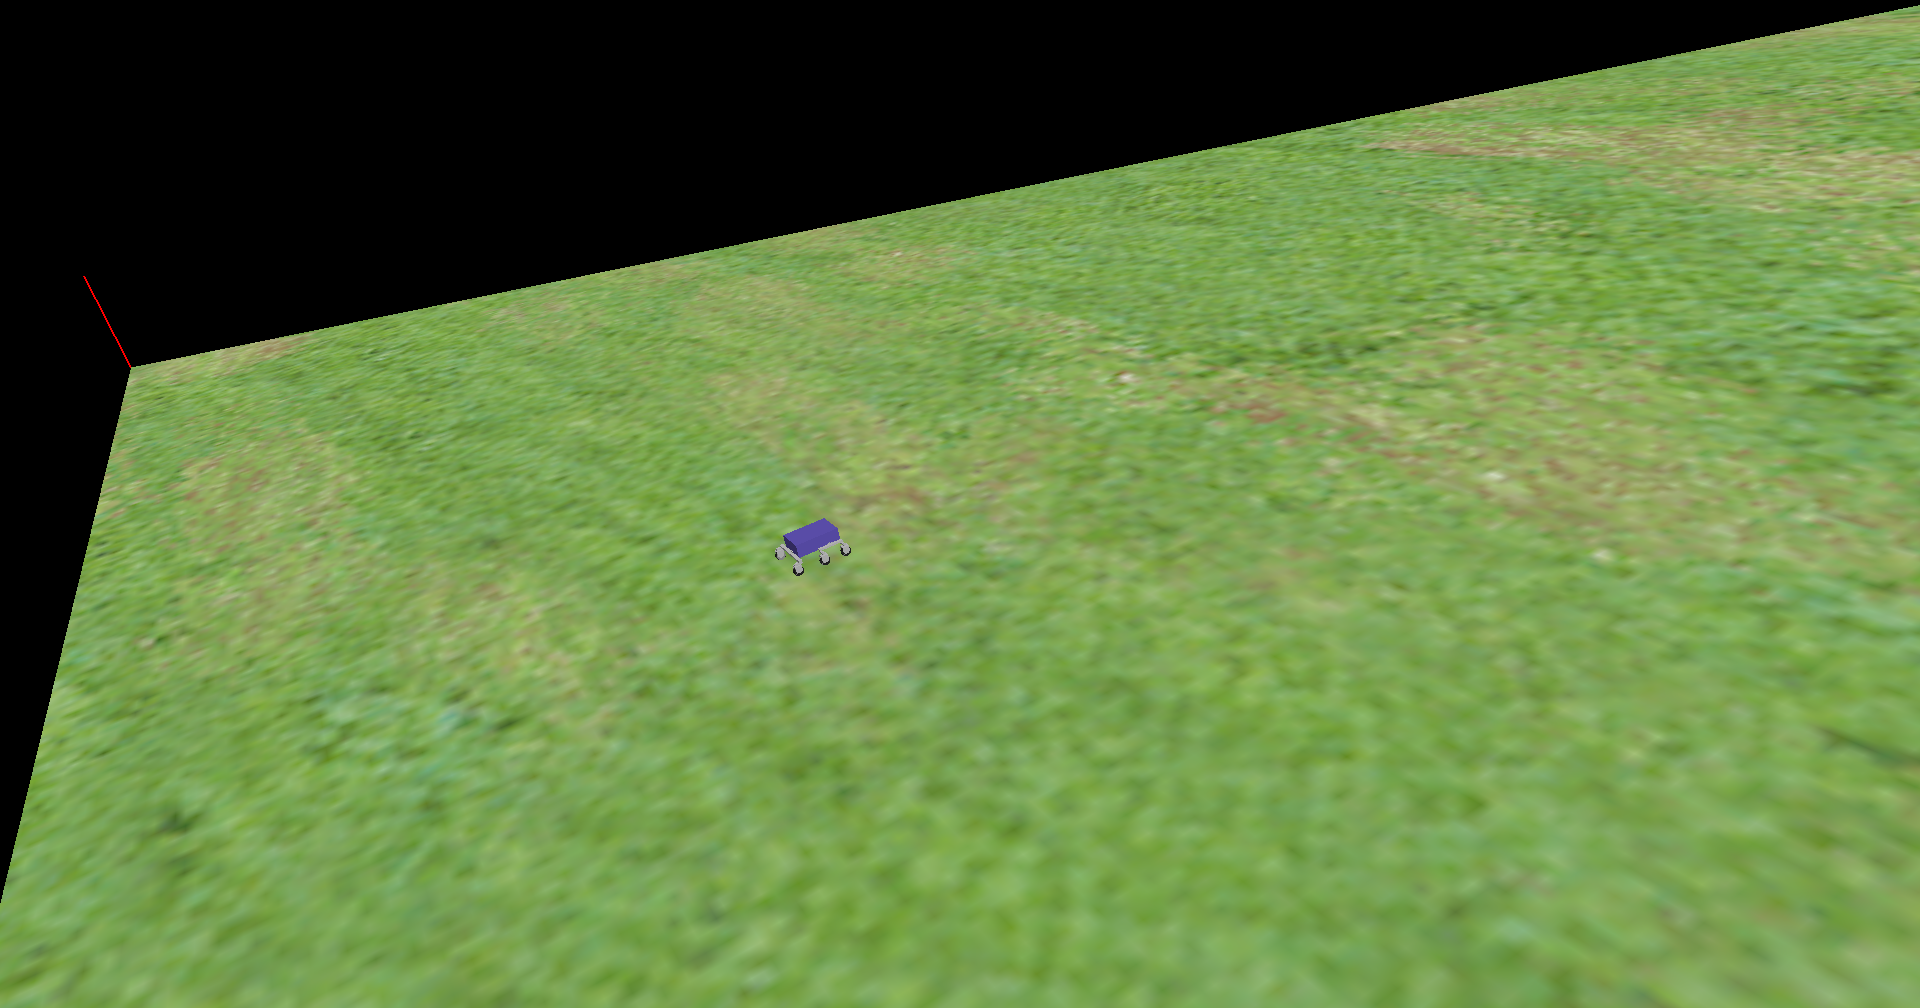
\includegraphics[width=0.8\textwidth]{run_5}
  \caption{Fifth test scenario}
\end{figure}

\noindent  In this setting we are mostly interested in two phases:

\begin{enumerate} 
  \item $119.965s < t_s < 200s$
  \item $200s < t_s < 300s$
\end{enumerate}

\noindent In this case, following quantities have been plotted:

\begin{itemize}
  \item $x_{COM}$ - mass center coordinates
\end{itemize}

\begin{figure}[H]
  \centering
    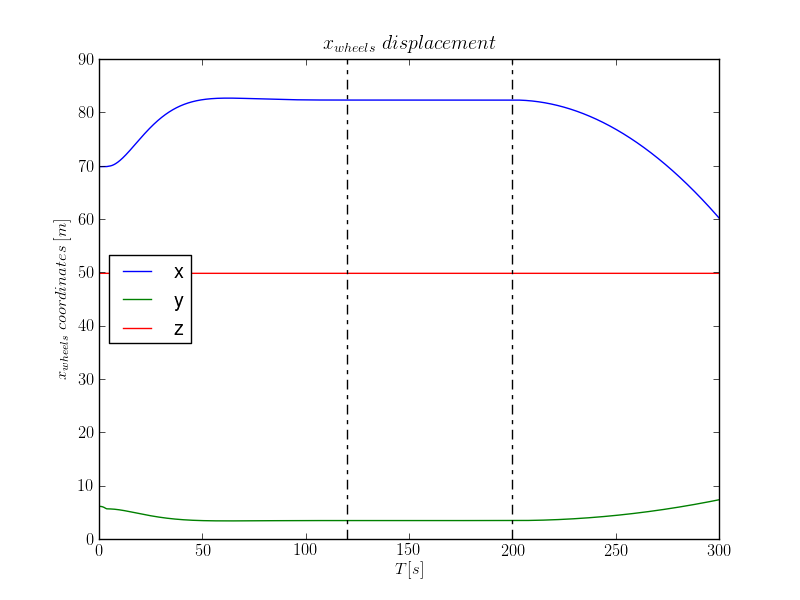
\includegraphics[width=0.8\textwidth]{xCOM5}
  \caption{$x_{COM}$}
\end{figure}

\begin{itemize}
  \item $x_{wheels}$ - wheels angular displacement 
\end{itemize}

\begin{figure}[H]
  \centering
    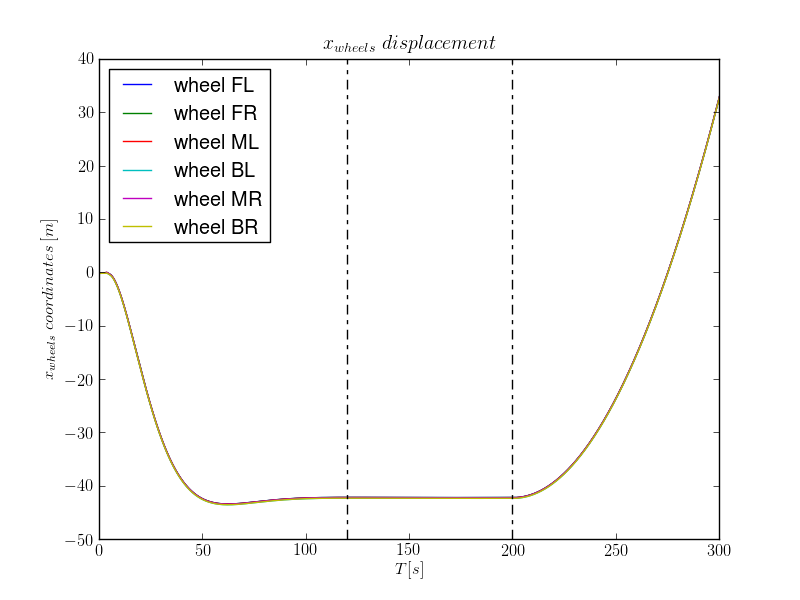
\includegraphics[width=0.8\textwidth]{xWHEELS5}
  \caption{$x_{wheels}$}
\end{figure}

\begin{itemize}
  \item $v_{COM}$ - mass center velocity
\end{itemize}

\begin{figure}[H]
  \centering
    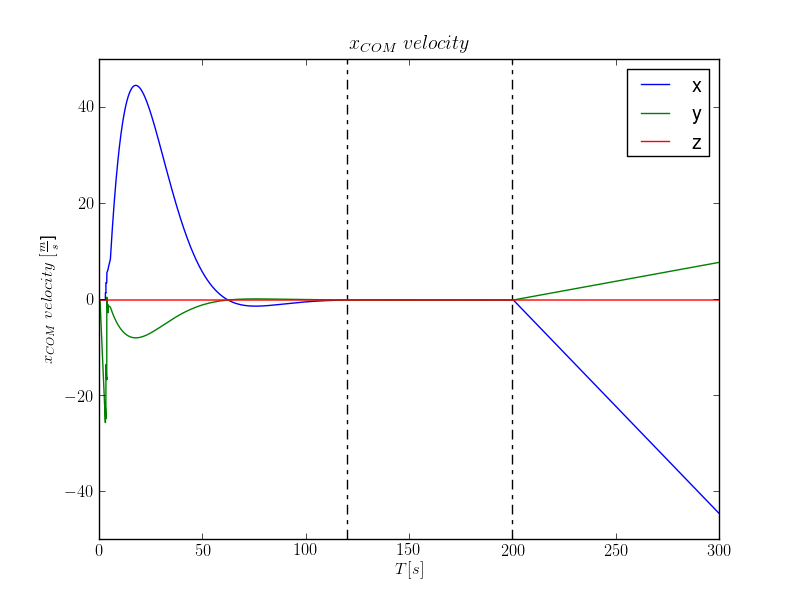
\includegraphics[width=0.8\textwidth]{vCOM5}
  \caption{$v_{COM}$}
\end{figure}

\begin{itemize}
  \item $v_{wheels}$ - wheels angular velocity
\end{itemize}

\begin{figure}[H]
  \centering
    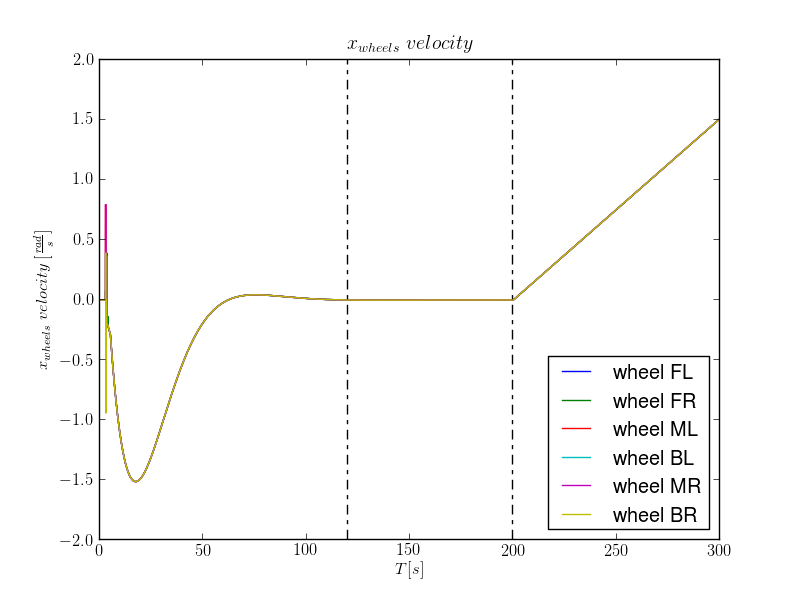
\includegraphics[width=0.8\textwidth]{vWHEELS5}
  \caption{$v_{wheels}$}
\end{figure}

\begin{itemize}
  \item $R_{COM}$ - reaction forces of center of mass in lagrangian coordinates
\end{itemize}

\begin{figure}[H]
  \centering
    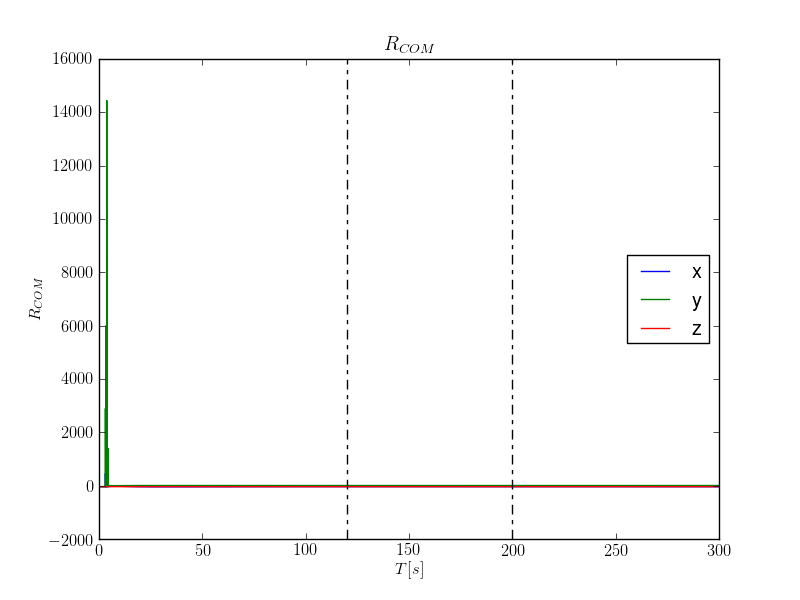
\includegraphics[width=0.8\textwidth]{pCOM5}
  \caption{$R_{COM}$}
\end{figure}

\begin{figure}[H]
  \centering
    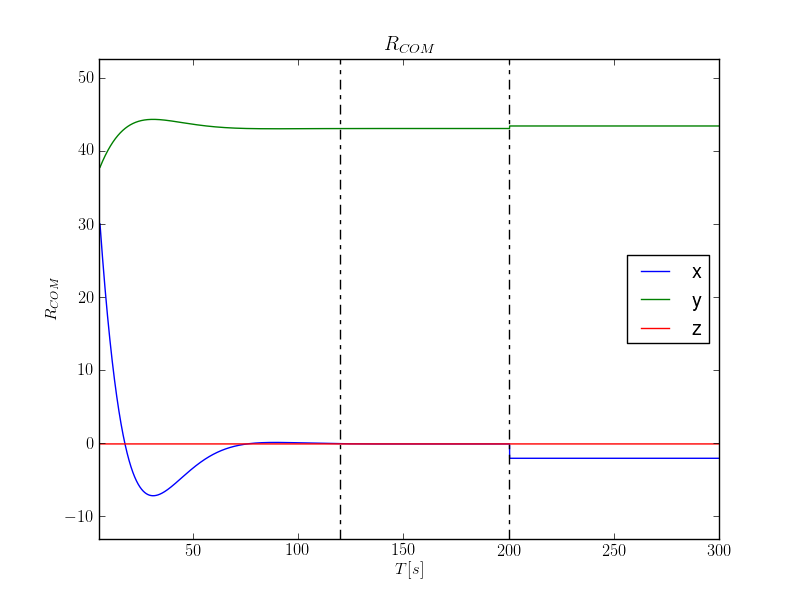
\includegraphics[width=0.8\textwidth]{pCOM5postimpact}
  \caption{$R_{COM}$ without impact part}
\end{figure}

\begin{itemize}
  \item $R_{wheels}$ - reaction forces of wheels in lagrangian coordinates
\end{itemize}

\begin{figure}[H]
  \centering
    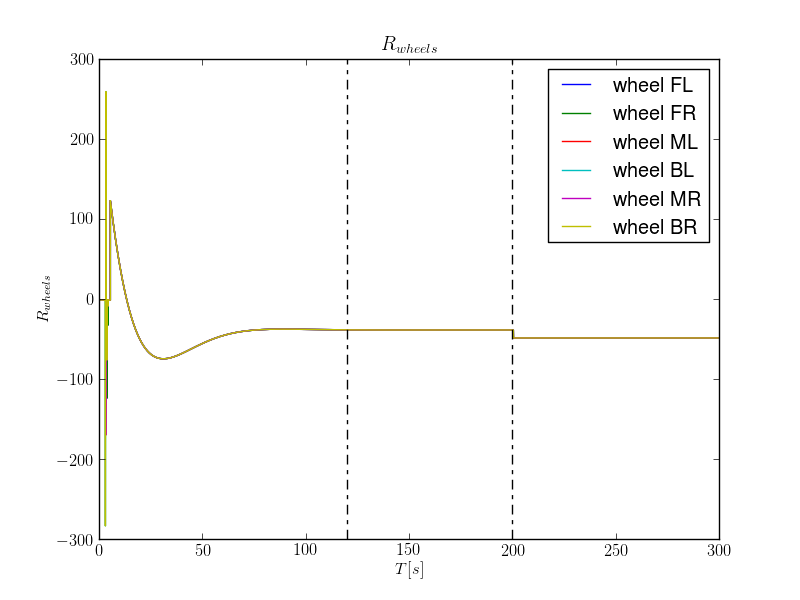
\includegraphics[width=0.8\textwidth]{pWHEELS5}
  \caption{$R_{wheels}$}
\end{figure}

\begin{itemize}
  \item $\lambda_{N}$ - normal component of the contact force (impulsion) for each wheel
\end{itemize}

\begin{figure}[H]
  \centering
    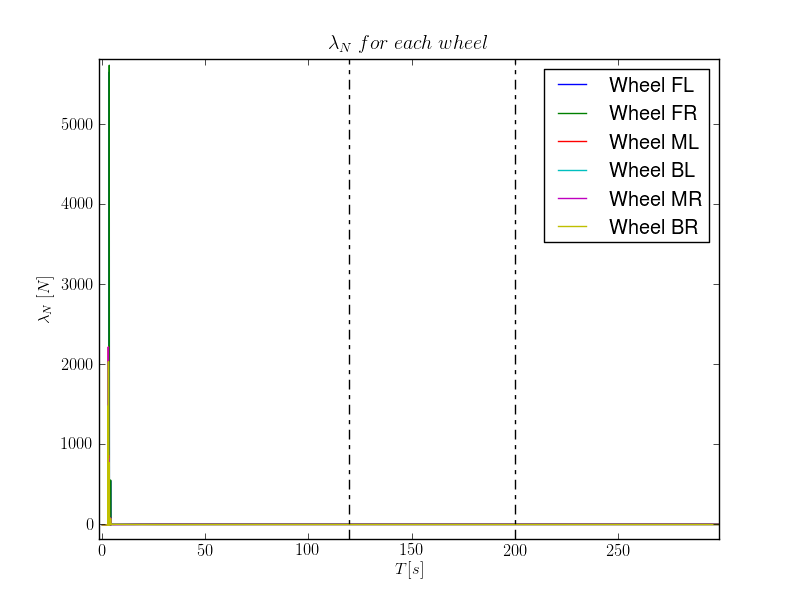
\includegraphics[width=0.8\textwidth]{lambdaN5}
  \caption{$\lambda_N$}
\end{figure}

\begin{figure}[H]
  \centering
    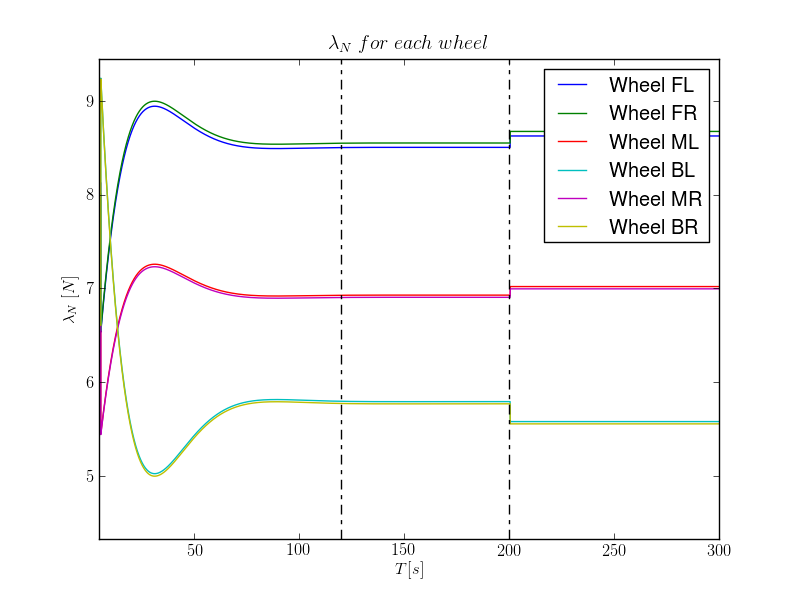
\includegraphics[width=0.8\textwidth]{lambdaN5zoom}
  \caption{$\lambda_N$ without impact phase}
\end{figure}

\begin{itemize}
  \item $\lambda_{T_x}$ - tangential component of the contact force in the x direction for each wheel
\end{itemize}

\begin{figure}[H]
  \centering
    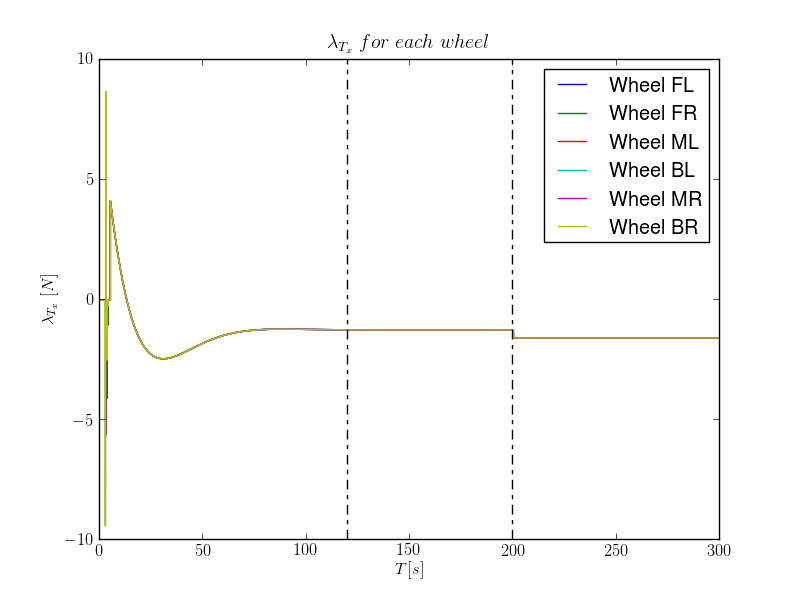
\includegraphics[width=0.8\textwidth]{lambdaTx5}
  \caption{$\lambda_{T_x}$}
\end{figure}

\begin{itemize}
  \item $\lambda_{T_z}$ - tangential component of the contact force in the z direction for each wheel
\end{itemize}

\begin{figure}[H]
  \centering
    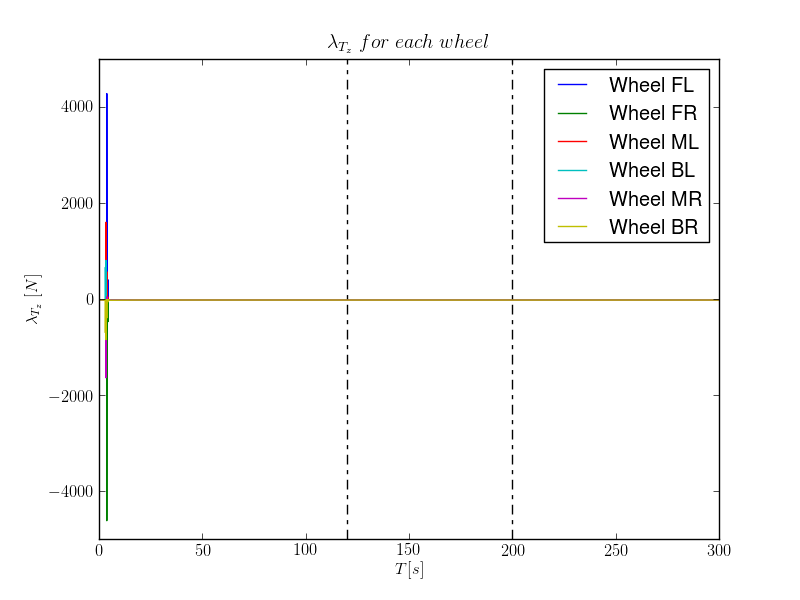
\includegraphics[width=0.8\textwidth]{lambdaTz5}
  \caption{$\lambda_{T_z}$}
\end{figure}

\begin{figure}[H]
  \centering
    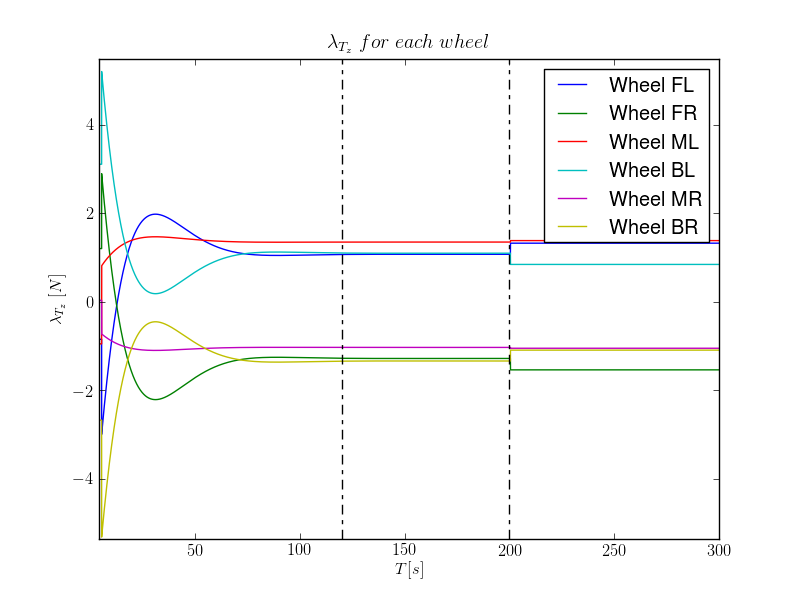
\includegraphics[width=0.8\textwidth]{lambdaTz5zoom}
  \caption{$\lambda_{T_z}$ without impact phase}
\end{figure}

\begin{itemize}
  \item $y_{N}$ - gap function (distance between contact point and the constraint function) for each wheel
\end{itemize}

\begin{figure}[H]
  \centering
    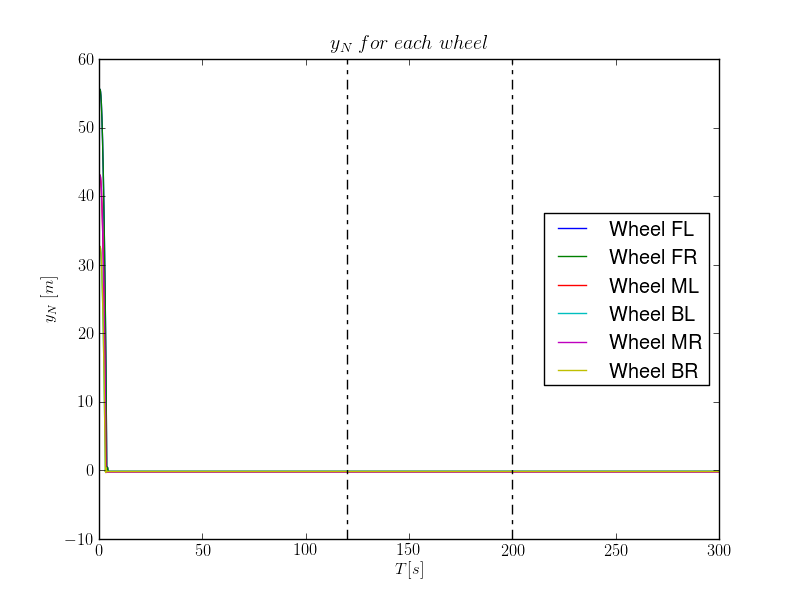
\includegraphics[width=0.8\textwidth]{yN5}
  \caption{$y_N$}
\end{figure}

\begin{figure}[H]
  \centering
    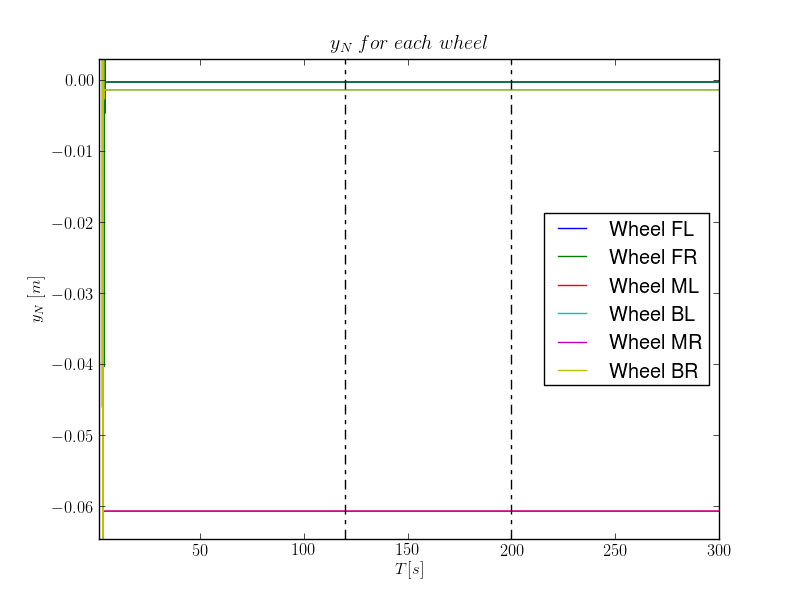
\includegraphics[width=0.8\textwidth]{yN5zoom}
  \caption{$y_N$ after impact phase}
\end{figure}

\begin{itemize}
  \item $\dot{y}_{N}$ - normal component of the local contact velocity for each wheel
\end{itemize}

\begin{figure}[H]
  \centering
    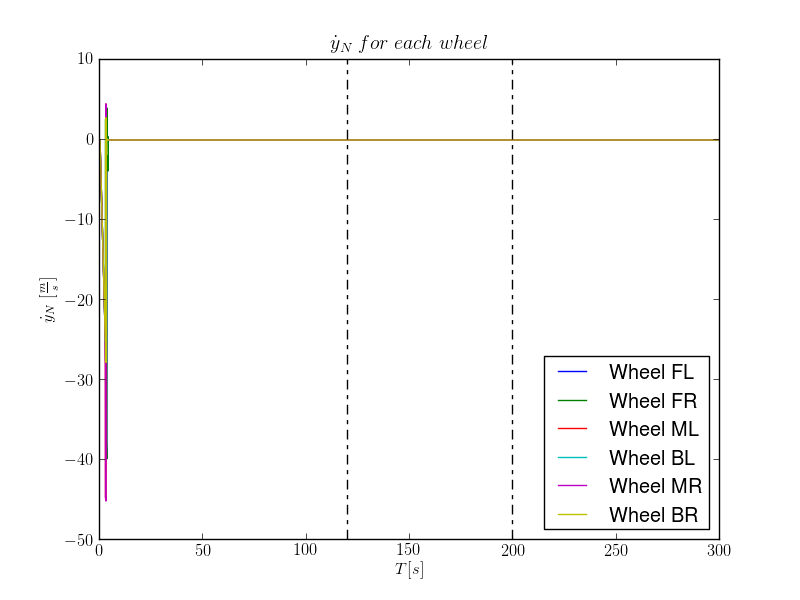
\includegraphics[width=0.8\textwidth]{yNdot5}
  \caption{$\dot{y}_{N}$}
\end{figure}

\begin{itemize}
  \item $\dot{y}_{T_x}$ - tangential component x of the local contact velocity for each wheel
\end{itemize}

\begin{figure}[H]
  \centering
    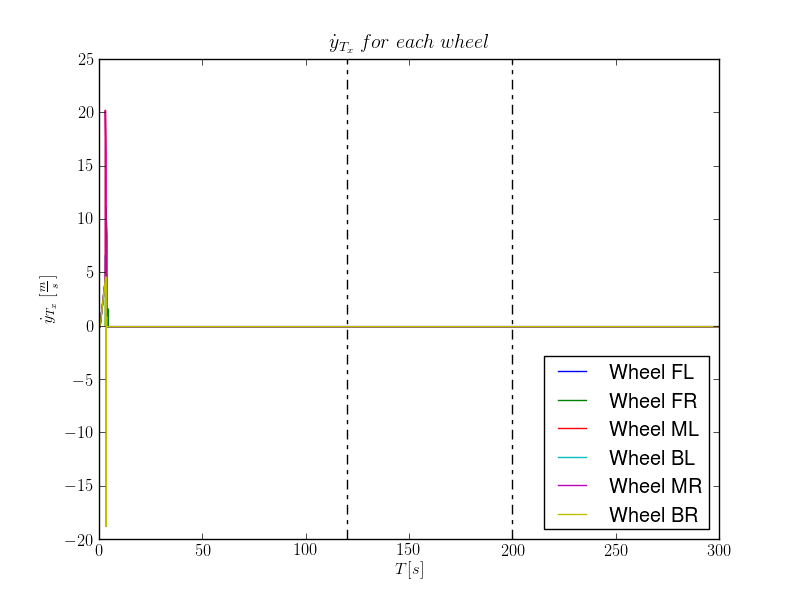
\includegraphics[width=0.8\textwidth]{yTxdots5}
  \caption{$\dot{y}_{T_x}$}
\end{figure}

\begin{itemize}
  \item $\dot{y}_{T_z}$ - tangential component z of the local contact velocity for each wheel
\end{itemize}

\begin{figure}[H]
  \centering
    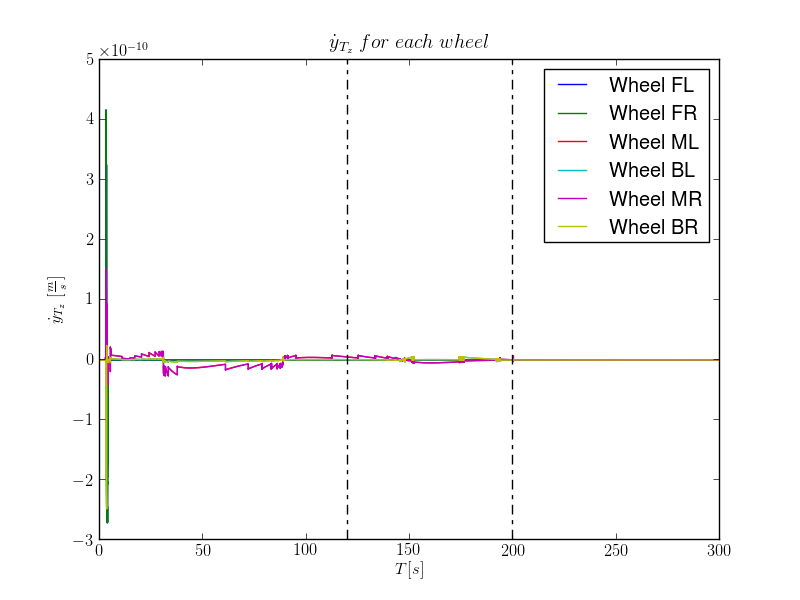
\includegraphics[width=0.8\textwidth]{yTzdots5}
  \caption{$\dot{y}_{T_z}$}
\end{figure}

